\subsubsection*{Вынужденные колебания под действием синусоидальной силы.}
Если в колебательный контур вставить последовательно источник переменного синусоидального напряжения, то получиться неоднородное уравнение, решением которого будут затухающие колебания + стационарное решение:
\begin{align*}
    U_c + \dot{U_c}CR + \ddot{U_c}CL = E\cos\omega t; \\
    U_c(t) = A_1e^{(-\gamma-\sqrt{\gamma^2-\omega_0^2})t}+A_2e^{(-\gamma+\sqrt{\gamma^2-\omega_0^2})t} + \frac{E\cos(\omega t + \arctan(R\omega C/(1-\omega^2 LC)))}{\sqrt{\omega^4L^2C^2+\omega^2(C^2R^2-2LC) + 1}}
\end{align*}
Чтобы не работать со столь сложными уравнениями можно прийти к простой идее, что стационарное решение в лучшем случае должно давать такие же синусоидальные колебания тока и напряжения на всех элементах цепи (предполагаем что такое решение уравнения в цепях есть всегда). В таком случае колебания напряжения и тока на элементе можно описать вращением постоянного по длине вектора в комплексной плоскости, ведь комплексная часть решения в уравнении слева и справа сокращается, что даёт нам возможность задать $Ecos\omega t$ так же вращающимся вектором $Ee^{i\omega t}$ (равенство векторов даёт равенство проекций на действительную ось, что нам и нужно). \newline
Заметим, что для конденсатора, индуктивности и резистора в случае гармонических колебаний выполняются обобщённые законы Ома:
$$
    U_c = -\frac{i}{\omega C}I_c;\;U_L = i\omega LI_L;\; U_R = RI_R\;(U_R,\;I_R, \;U_c,\;I_c,\;U_L,\;I_L\text{\;комлексные\;в\; общем\;случае})
$$
Данный факт позволяет нам складывать импедансы ("сопротивления"$\;$элементов в общем случае) параллельно и последовательно также как и для резисторов.
Таким образом получаем:
$$
    E = I\cdot(R + i\omega L - \frac{i}{\omega C});\;|E| = |I|\cdot|(R + i\omega L - \frac{i}{\omega C})|;
$$
Таким образом легко получит сдвиг фаз как угол между векторами $E$ и $I$: $\varphi = \arctan(R\omega C/(1-\omega^2 LC))$
\newline
\subsubsection*{Амплитудная и фазовая характеристики. Резонанс.}
Найдём зависимости амплитуды $U_c$, $U_L$ и $I$ в контуре от частоты:
\begin{align*}
U_c &= E/\sqrt{\omega^4L^2C^2+\omega^2(C^2R^2-2LC) + 1}; \\
U_L &= E/\sqrt{(1-\frac{1}{\omega^2LC})^2 + \frac{R^2}{\omega^2L^2}}; \\
I &= E/\sqrt{R^2+(\omega L - 1/(\omega C))^2}
\end{align*}
\begin{center}
    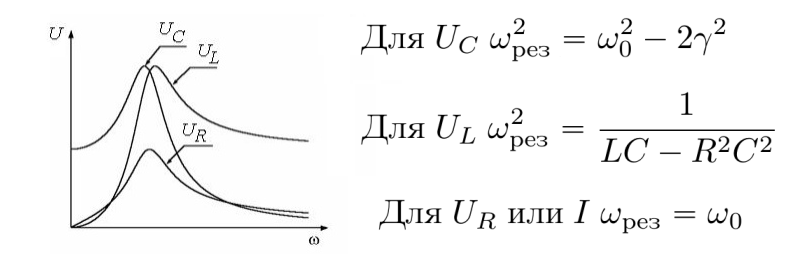
\includegraphics[scale=0.5]{img/resonance.png}
\end{center}
Важно заметить, что частоты эти не совпадают и даже не всегда существуют.
\newline
Найдём фазовочастотные характеристики для $U_c$, $U_L$ и $I$ в контуре:
$$\phi_c = -arctan(R\omega C/(1-\omega^2 LC));\;\phi_I = arctan((1-\omega^2 LC)/R\omega C);\; \phi_L = -arctan(R\omega C/(1-\omega^2 LC)) = \pi+\phi_c;$$
\begin{center}
    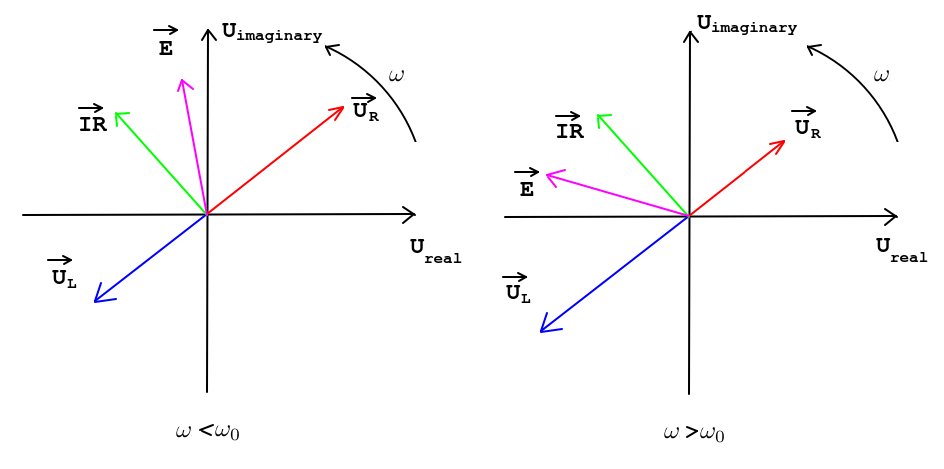
\includegraphics[scale=0.5]{img/vectors.png}
\end{center}
\subsubsection*{Ширина резонанса и ее связь с добротностью.}
Формулу для тока в RLC цепи можно переписать как:
$$I = \frac{E/(2\gamma L)}{\sqrt{1+(\frac{\omega_0}{\omega} - \frac{\omega}{\omega_0})^2(\frac{\omega_0}{2\gamma})^2}};\;I_{\text{рез}} = E/R$$
Тогда если использовать формулу для добротности свободных колебаний (и так сойдёт!):
$$\frac{I}{I_{\text{рез}}} = \frac{1}{\sqrt{1+(\frac{\omega_0}{\omega} - \frac{\omega}{\omega_0})^2Q^2}}$$
А если ещё $\frac{\Delta\omega}{\omega_0} = \frac{|\omega - \omega_0|}{\omega_0} \ll 1$ и $Q \gg 1$ (иначе формулу для добротности нельзя было использовать):
$$\frac{I}{I_{\text{рез}}} = \frac{1}{\sqrt{1+(\frac{2\Delta\omega}{\omega_0})^2Q^2}}$$
Наложим условие и найдём соотношение для ширины кривой и добротности:
$$\frac{I}{I_{\text{рез}}} =1/\sqrt{2};\;Q=\frac{\omega_0}{2\Delta\Omega}$$
В параллельном контуре при приближении к резонансу $\omega = \omega_0$ резко возрастает сопротивление, так что удобнее было бы рассматривать зависимость напряжение на цепи в зависимости от частоты при подключённом источнике синусоидального тока (амплитуда тока постоянна). В таком случае форма резонансной кривой и её ширина такая же как и в рассмотренном выше случае
\newline
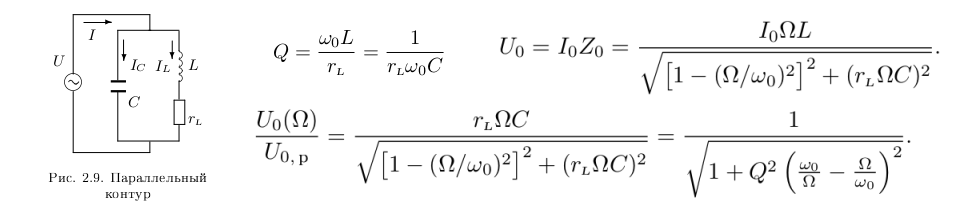
\includegraphics[scale=0.6]{img/ParCircuit.png}
\subsubsection*{Процесс установления вынужденных колебаний, биения.}
Процесс установления колебаний это вынужденные колебания + затухающие (свободные). Всерьёз находить эти коэффициенты из начальных условий вас вряд ли заставят.
\newline
Биения возникают при сложении очень близких по частоте колебаний. Например, когда в RLC цепи начинают подавать сигнал, близкий к резонансному. В таком случае складываются затухающие и стационарные колебания.
\newline
Если подать сигнал с частотой, очень близкой к резонансной, то биения не будут видны, так как разность фаз между сигналами не успеет сильно вырасти за характерное время затухания свободных колебаний.
Условие возникновения биений:
$$\Delta\omega \ll \frac{\omega}{Q},
\hspace{0.5cm} \Rightarrow \hspace{0.5cm} 
U = U_0(1-e^{-\gamma t})cos(\omega_0t-\phi);\;\;\theta = \frac{1}{n}ln\frac{U_0-U_k}{U_0-U_{k+n}}.
$$
